\documentclass{BeamerTemplate}

\usepackage{ulem}

\title{Module 6 - Lois échantillonnales et estimation ponctuelle}

\date{\today}
\graphicspath{{Images/Module 6/}}

\begin{document}
\begin{frame}[t]
  \titlepage
\end{frame}

%-------------------------------------------------------------------------------------------------------------------------------------





%%%%%%%%%%%%%%%%%%%%%%%%%%%%%%%%%%%
%%%%%%%%%%%%%%%%%%%%%%%%%%%%%%%%%%%
%%%%%%%%%%%%%%%%%%%%%%%%%%%%%%%%%%%


\section{Concepts d'inférence statistique}


\begin{frame}[t]{L'inférence statistique}

Tirer des conclusions au sujet d'une population à l'aide d'un échantillon.\\

\begin{itemize}\itemsep 5mm
\item<2-> Produire 50 pièces avec une certaine machine pour vérifier la variabilité de la taille des pièces.
\item<2-> Soumettre une douzaine de câbles d'un nouveau type à un test de résistance pour confirmer
qu'il peuvent, en moyenne, soutenir une masse de 10 tonnes.
\item<2-> Sonder des étudiants afin de déterminer si le LPU les intéresse.

\end{itemize}

\vfill
\uncover<3->{\alert{Important}: Il faudra se rappeler qu'à partir de maintenant, les paramètres des lois (par exemple $\mu$ dans le cas d'une loi normale) représentent des attributs de la population qui nous intéressent, mais \alert{leur valeur est \textbf{inconnue}} et nous voulons l'estimer.}
\end{frame}

% \begin{frame}[t]{Deux types d'inférence}

% \begin{tabular}{p{5cm}|p{5cm}}
% {\bf Estimation de paramètres}&{\bf Vérification d'hypothèses}\\\hline

% \uncover<2->{\alert{Estimation ponctuelle:} }& \uncover<4->{\alert{Tests d'hypothèses:} }\\[3mm]
% \uncover<2->{$\bullet\;\mu$ estimé par $\overline{X}$}&\uncover<4->{$\bullet\;$ A-t-on $\;\mu\leq60$?} \\[3mm]
% \uncover<2->{$\bullet\;\sigma^2$ estimé par $S^2$}&\uncover<4->{$\bullet\;$ A-t-on $\;\sigma^2<10$?}\\[3mm]\cline{1-1}
% \uncover<3->{\alert{Intervalles de confiance: }}&\uncover<4->{$\bullet\;$ A-t-on $\;\mu_1=\mu_2=\mu_3 $?}\\[3mm]
% \uncover<3->{associer une marge d'erreur}&\\[-1mm]
% \uncover<3->{aux estimations ponctuelles}
% \end{tabular}

% \end{frame}

\begin{frame}[t]{Deux types d'inférence}

\renewcommand{\arraystretch}{1.5}

\begin{tabularx}{\textwidth}{|>{\raggedright\arraybackslash}X|>{\raggedright\arraybackslash}X|}
  \toprule
  \textbf{Estimation de paramètres} & \textbf{Vérification d’hypothèses (modules 8.1 et 8.2)} \\
  \midrule
  \textcolor{red}{\textbf{Estimation ponctuelle (module 6):}}  
  \newline Un ou plusieurs paramètres estimés par une fonction de l’échantillon 
  & 
  \multirow{2}{=}{%
    \textcolor{red}{\textbf{Tests d’hypothèses  :}}\newline
    \begin{itemize}
      \setlength\itemsep{0.4em}
      \item A-t-on \( \mu \geq 10 \) ?
      \item A-t-on \( \sigma^2 < 25 \) ?
      %\item A-t-on \( \mu_1 = \mu_2 = \mu_3 \) ?
    \end{itemize}
  } \\
  \cmidrule{1-1}
  \textcolor{red}{\textbf{Intervalles de confiance (module 7):}} 
  \newline Associer une marge d’erreur aux estimations ponctuelles & \\
  \bottomrule
\end{tabularx}

\end{frame}

\section{Échantillons aléatoires et statistiques}

\begin{frame}{Échantillon aléatoire}
\begin{Boite}{Échantillon aléatoire}
    Soit $X$, une variable aléatoire de répartition $F_X$. Si tous les résultats de l'ensemble $X_1,\hdots,X_n$ ont été obtenus de manière aléatoire et indépendante, on dit que $X_1,\hdots,X_n$ est un \alert{échantillon aléatoire}.
\end{Boite}



   En pratique, on a une grande (voire infinie) population d'objets ou d'individus et la valeur de $X$ varie d'un individu à l'autre dans la population selon $F_X$. On choisit au hasard $n$ individus dans cette population et les valeurs $X_1,\dots,X_n$ de $X$ que l'on obtient est un échantillon aléatoire.

    
\end{frame}


\begin{frame}{Statistique}
\begin{Boite}{Statistique}
    Une fonction $T(X_1,\hdots,X_n)$ qui n'est pas dépendante de paramètres inconnus est appelée \alert{statistique}.
\end{Boite}
    

    Une statistique est donc tout simplement une valeur que l'on peut calculer à partir d'un échantillon.


\end{frame}

\begin{frame}{Deux exemples de statistiques}
    Soit $X_1,\hdots,X_n$, un échantillon aléatoire provenant de $X$, une certaine variable aléatoire. La moyenne échantillonnale et la variance échantillonnale sont deux exemples de statistiques qu'il est possible de calculer à partir des valeurs $X_1,\dots,X_n$ :

    \begin{align*}
        \overline{X}=\frac{1}{n}\sum_{i=1}^n X_i & & S^2=\frac{1}{n-1}\sum_{i=1}^n(X_i-\overline{X})^2
    \end{align*}

    %Comme les différentes statistiques sont des fonctions de variables aléatoires, elles sont des \alert{variables aléatoires}.
    
\end{frame}

\begin{frame}[t]{Valeur de statistiques}
    
\centerline{\LARGE\bf\alert{QUIZ !}}

  \vspace{2mm}
  Je tire un échantillon aléatoire $X_1,\dots,X_{16}$ d'une population dans laquelle la valeur de $X$ suit une loi normale d'espérance
  10 et de variance 4. Je calcule la moyenne échantillonnale de l'échantillon. On dénote la valeur que j'obtiens $\overline{X}^A$.

  Mon meilleur ami tire ensuite lui aussi un échantillon aléatoire de taille 16 de cette même population. Il en calcule la moyenne échantillonale, que l'on dénote $\overline{X}^B$.

  {\bf Question :\ } Que peut-on dire des valeurs $\overline{X}^A$ et $\overline{X}^B$ ?
  \begin{enumerate}
      \item[(a)] Elles sont toutes deux égales à 10.
      \item[(b)] Elles sont toutes deux égales, mais pas nécessairement égales à 10.
      \item[(c)] Elles prennent des valeurs différentes l'une de l'autre, mais probablement <<pas trop éloignées>> de 10.
  \end{enumerate}
 \vspace{5cm}
\end{frame}

\begin{frame}[t]{Valeur de statistiques}
    
\centerline{\LARGE\bf\alert{QUIZ !}}

  \vspace{2mm}
 
\vfill
    \href{https://jmiron-moyechnorm.share.connect.posit.cloud/}{Simulons cette expérience !}
    
\end{frame}


% \section{La moyenne échantillonnale}
% \begin{frame}[t]{Moyenne échantillonnale}
% Soit l'échantillon aléatoire  $X_1,\hdots,X_n$ d'une certaine variable aléatoire $X$ pour laquelle $E(X)=\mu$ et $V(X)=\sigma^2$.

% Sachant que $$\overline{X}=\frac{1}{n}\sum_{i=1}^nX_i,$$

% il est possible de montrer que $E(\overline{X})=\mu$ et $\displaystyle V(\overline{X})=\frac{\sigma^2}{n}$.

% \vspace{0.5cm}
% \alert{$\rightarrow$ Il s'agit d'une variable aléatoire!}

% \vfill
%     \href{https://jmiron-estimation-ponctuelle.share.connect.posit.cloud/}{Exemple quand $X\sim\mathcal{N}(\mu,\sigma^2)$.}
% \end{frame}

% \section{La variance échantillonnale}

% \begin{frame}[t]{Variance échantillonnale}
%  Soit l'échantillon aléatoire  $X_1,\hdots,X_n$ d'une certaine variable aléatoire $X$ pour laquelle $E(X)=\mu$ et $V(X)=\sigma^2$.

% Sachant que $$S^2=\frac{1}{n-1}\sum_{i=1}^n(X_i-\overline{X})^2,$$

% il est possible de montrer que $E(S^2)=\sigma^2$ et que si $X\sim\mathcal{N}(\mu,\sigma^2)$, $\displaystyle V(S^2)=\frac{2\sigma^4}{n-1}$.

% \vspace{0.5cm}
% \alert{$\rightarrow$ Il s'agit d'une variable aléatoire!}   
% \end{frame}

\begin{frame}[t]{Comportement des statistiques}
  Soit $X_1,\dots,X_n$ un échantillon aléatoire, et considérons
  la valeur d'une statistique calculée à partir de cet échantillon, disons $Y=T(X_1,\dots,X_n)$.

  Le quiz précédent nous fait réaliser que \alert{$Y$ est aussi une {\bf variable aléatoire}} !

\vspace{1cm}
    Le concept de variable aléatoire est très important pour les modules qui suivront.

    \medskip
    Il faut donc d'ores et déjà comprendre que $\overline{X}$, par exemple, dépend de l'échantillon et prendra \alert{assurément} une valeur différente dans un échantillon différent. 

\end{frame}

%%%%%%%%%%%%%%%%%%%%%%%%%%%%%%%%%%%%%%%%%%%%%%%%%%%%%%%%%%%%%%%%%%%%%%%%%%

\section{Lois échantillonnales}

\begin{frame}[t]{Distribution de certaines statistiques}
\begin{enumerate}[$\bullet$]
\item Les statistiques sont des \alert{variables aléatoires}.
\item Leur loi dépend de la loi de $X$ dans la population.
 \item Les lois qui décrivent le comportement aléatoire de statistiques sont appelées des {\it lois échantillonnales}. %Nous en verrons quatre:
%     \begin{itemize}\itemsep1mm
% \item Normale $N(\mu, \sigma^2/n)$
% \item Khi-carré $\chi^2_v$
% \item Student $\;\;t_v$
% \item Fisher $\quad F_{u,v}$
%\end{itemize}
\item Nous allons étudier les lois échantillonnales reliées à $\overline{X}$ et $S^2$.
\end{enumerate}

\end{frame}

\section{La moyenne échantillonnale}
\begin{frame}[t]{Moyenne échantillonnale}
Soit l'échantillon aléatoire  $X_1,\hdots,X_n$ d'une certaine variable aléatoire $X$. 
On ne fait aucune supposition sur la loi de $X$, sauf que $E(X)=\mu$ et $V(X)=\sigma^2$.

Comme $$\overline{X}=\frac{1}{n}\sum_{i=1}^nX_i,$$

il est possible de montrer que $E(\overline{X})=\mu$ et $\displaystyle V(\overline{X})=\frac{\sigma^2}{n}$.

\vspace{0.5cm}
\vfill
    \href{https://jmiron-moyechexp.share.connect.posit.cloud/}{Simulation.}
\end{frame}

\section{La variance échantillonnale}

\begin{frame}[t]{Variance échantillonnale}
Soit l'échantillon aléatoire  $X_1,\hdots,X_n$ d'une certaine variable aléatoire $X$. 
On ne fait aucune supposition sur la loi de $X$, sauf que $V(X)=\sigma^2$.

On se souvient que $$S^2=\frac{1}{n-1}\sum_{i=1}^n(X_i-\overline{X})^2.$$

Il est possible de montrer que nous avons toujours $E(S^2)=\sigma^2$ et que si $X_1,\hdots,X_n$ sont normaux, $\displaystyle V(S^2)=\frac{2\sigma^4}{n-1}$.

\vspace{1cm}
\href{https://jmiron-moyechexp.share.connect.posit.cloud/}{Simulation.}

\end{frame}

\section{Échantillons aléatoires d'une population $\mathcal{N}(\mu,\sigma^2)$}

\begin{frame}[t]{Cas très commun}
    On peut déterminer la distribution complète (pas seulement l'espérance ou la variance) 
    de $\overline{X}$ et de $S^2$ dans le cas particulier où $X_1,\dots,X_n$ est un échantillon
    aléatoire d'une loi $\mathcal{N}(\mu,\sigma^2)$.
\end{frame}

\begin{frame}[t]{Distribution de $\overline{X}$ dans le cas normal}
\begin{Boite}{Distribution de $\overline{X}$ dans le cas normal}
    Soit $X_1,\dots,X_n$, un échantillon aléatoire d'une loi $\mathcal{N}(\mu,\sigma^2)$. Alors dans ce cas
    il est possible de démontrer que
    $$\overline{X}\sim \mathcal{N}\left(\mu,\frac{\sigma^2}{n}\right).$$    
\end{Boite}

   \uncover<2->{
\vspace{0.5cm}
\vfill
    \href{https://jmiron-moyechnorm.share.connect.posit.cloud/}{P.ex., si $\mu=10$, $\sigma^2=4$ et $n=16$, alors $\overline{X}\sim\mathcal{N}(10,4/16)$ ... simulons !}
   }
\end{frame}

\begin{frame}[t]{Standardisation}
  De la page précédente et des propriétés de la loi normale, on peut déduire que
  $$Z=\frac{\overline{X}-\mu}{\sigma/\sqrt{n}}\sim\mathcal{N}(0,1).$$

  \medskip

  {\bf Remarque :} La variable $Z$ définie ci-dessus n'est pas une statistique quand
  $\mu$ et $\sigma^2$ sont inconnues, mais elle l'est dans les cas où l'on connaît ou l'on
  fixe des valeurs pour $\mu$ et $\sigma^2$.

  \vspace{0.5cm}
\vfill
    \href{https://jmiron-moyechnorm.share.connect.posit.cloud/}{Retour à la simulation ...}
\end{frame}





\section{Loi du khi-carré}

\begin{frame}{Loi échantillonnale de $S^2$}
   Pour discuter du comportement aléatoire de $S^2$, il faut introduire une nouvelle loi de probabilité.
\end{frame}

\begin{frame}[t]{Loi du khi-carré (khi-deux): $\chi^2_v$}

\begin{itemize}
%\item loi pour les variables aléatoires continues
\item valeurs possibles d'une variable suivant une $\chi^2_v$ : $[0,\infty)$ %Elle est fortement liée à la loi gamma.
\item un seul paramètre qu'on appelle "degrés de liberté".
\end{itemize}

\begin{center}
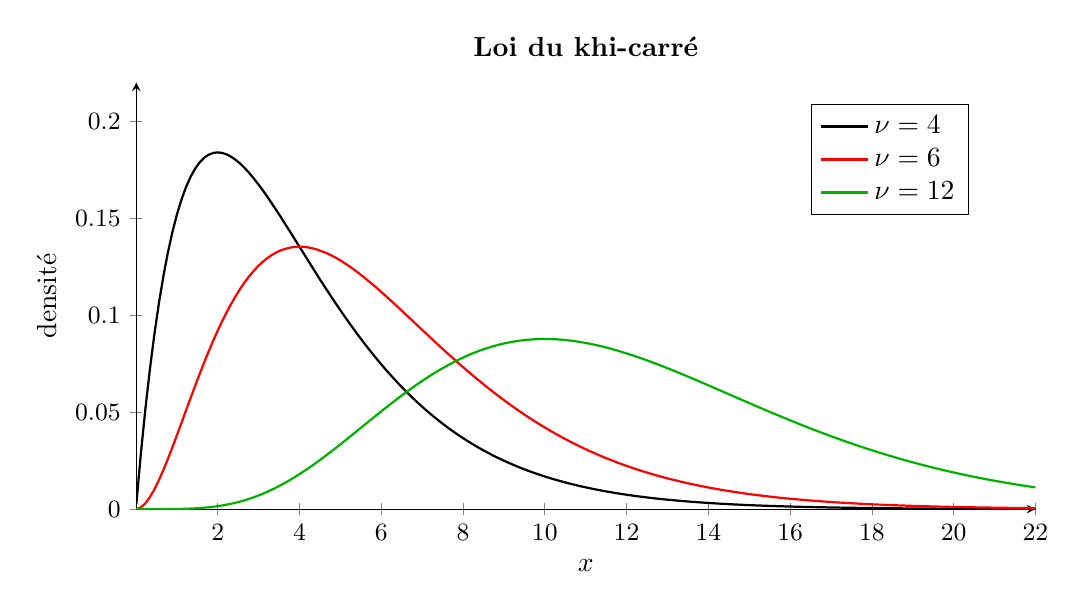
\begin{tikzpicture}
\begin{axis}[
    domain=0.01:22,
    samples=200,
    axis lines=left,
    ymin=0, ymax=0.22,
    xlabel={$x$},
    ylabel={densité},
    ytick={0, 0.05, 0.10, 0.15, 0.20},         % <--- Forçage des valeurs
    yticklabel style={/pgf/number format/fixed},    % <--- Affichage décimal forcé
    scaled y ticks=false,                           % <--- Pas de notation scientifique
    legend style={draw=black, fill=white, at={(0.75,0.95)}, anchor=north west},
    title={\textbf{Loi du khi-carré}},
    width=13cm,
    height=7cm,
    tick label style={font=\small},
    legend cell align={left}
]

% courbes des densités
\addplot[black, thick] {0.25 * x * exp(-x/2)};
\addlegendentry{$\nu=4$}

\addplot[red, thick] {x^2 * exp(-x/2)/16};
\addlegendentry{$\nu=6$}

\addplot[green!70!black, thick] {x^5 * exp(-x/2)/7680};
\addlegendentry{$\nu=12$}

\end{axis}
\end{tikzpicture}
\end{center}
\end{frame}

\begin{frame}[t]{Propriétés de la loi du khi-carré}

{\small
\begin{itemize}\itemsep2mm
\item Si $K\sim\chi^2_v$, alors $\left\{\begin{array}{ll}E(K)& = v\\V(K) &= 2v
    \end{array}\right.$
\item Si $Z\sim N(0,1)$, alors $Z^2\sim\chi^2_1$ %[et donc si $Z\sim N(\mu,\sigma^2)$ et $X = \{(Z-\mu)/\sigma\}^2$, alors $X\sim\chi^2_1$].
\item Si $K_1,\ldots,K_n$ sont des v.a. indépendantes et que $K_i\sim\chi^2_{v_i}$, alors $$K_1+\cdots+K_n\sim\chi^2_{v_1+\cdots+v_n}$$
\item Si $X_1,\ldots,X_n$ sont i.i.d. $N(\mu,\sigma^2)$, alors $$\dfrac{\sum_{i=1}^n(X_i-\mu)^2}{\sigma^2}\sim\chi^2_n $$ %\qquad \text{et}\qquad\frac{(n-1)S^2}{\sigma^2}\sim\chi^2_{n-1}$$
\end{itemize}
}

\href{https://jmiron.shinyapps.io/KhiCarre/}{Génération de khi-carré.}
\end{frame}

\begin{frame}[t]{Table de la loi du khi-carré}


\begin{minipage}[b]{2.5cm}{
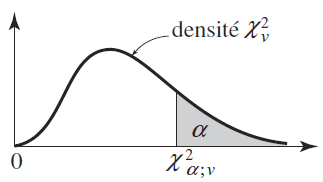
\includegraphics[width=2.5cm]{khi-fig.PNG}

\vspace{9cm}}
\end{minipage}
\begin{minipage}[b]{7.6cm}{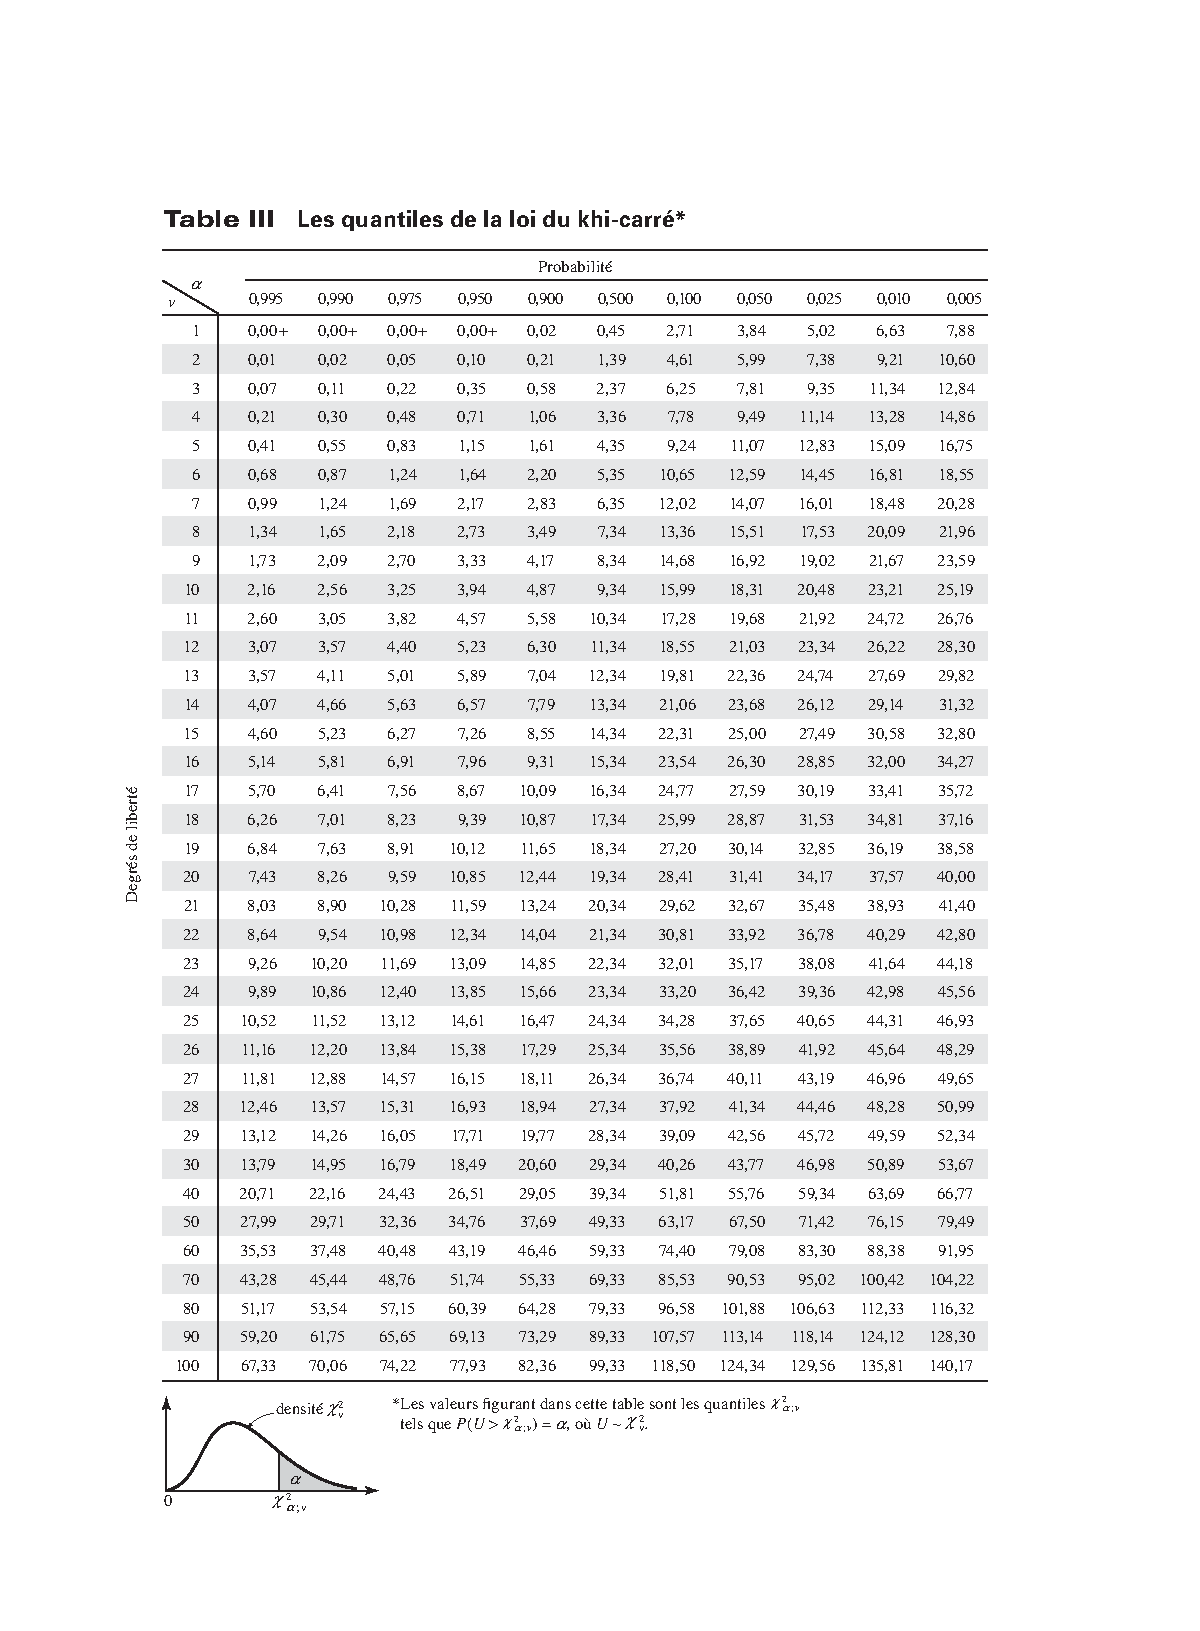
\includegraphics[width=7.6cm]{table_khi2.pdf}} \end{minipage}

\end{frame}

\begin{frame}[t]{Loi échantillonnale de $S^2$}
   Il est possible de démontrer que les propriétés précédentes mènent au résultat qui suit.
   \begin{Boite}{Loi échantillonnale de $S^2$}
    Soit $X_1,\dots,X_n$ un échantillon aléatoire d'une loi $\mathcal{N}(\mu,\sigma^2)$. Alors
    $$\frac{(n-1)S^2}{\sigma^2}\sim\chi^2_{n-1}.$$
\end{Boite}
 
\end{frame}

\begin{comment}
\uncover<2->{
On cherche $P[S^2 > 54,4]$. Comme les températures sont i.i.d. $N(\mu,\sigma^2)$, on
sait que $\frac{(n-1)S^2}{\sigma^2}\sim\chi^2_{n-1}$.
}

 Donc
\begin{align*}
P[S^2 > 54,4] &= P\left[\frac{(n-1)S^2}{\sigma^2} > \frac{(n-1)54,4}{\sigma^2}\right]\\
&= P\left[\frac{19S^2}{38}>\frac{(19)(54,4)}{38}\right]\\
&= P\left[\chi^2_{19} > 27,2\right],
\end{align*}
et cette probabilité est 0,10 selon la table du khi-carré de la p. 478.
%%%%%%%%%%%%%%%%%%%%%%%%%%%%%%%%%%%%%%%%%%%%%%%%%%%%%%%%%%%%%%%%%%%

png("khi.png",width=6,height=4,unit="in",res=90)
par(mar=c(2,3,1,1))
x<-seq(0,22,length=1000)
plot(x,dchisq(x,3), type="l", main="Loi du khi-carré",xlab="u",ylab="Densité",ylim=c(0,0.25),col=1,lwd=3,las=1,yaxs="i",bty="l")
par(new=TRUE)
plot(x,dchisq(x,6), type="l",ylab=" ",xlab="",ylim=c(0,0.25),col=2,lwd=3,las=1,yaxs="i",bty="l")
par(new=TRUE)
plot(x,dchisq(x,12), type="l",ylab=" ",xlab="",ylim=c(0,0.25),col=3,lwd=3,las=1,yaxs="i",bty="l")
text<-c("v=3","v=6","v=12")
legend("topright",text,col=1:3,lty=1,lwd=3,cex=1.2)
dev.off()

png("t.png",width=6,height=4,unit="in",res=90)
par(mar=c(2,3,1,1))
x<-seq(-4,4,length=1000)
plot(x,dt(x,3), type="l", main="Loi de Student",ylab="Densité",xlab="t",ylim=c(0,0.5),col=1,lwd=2,las=1,yaxs="i",bty="l")
par(new=TRUE)
plot(x,dt(x,6), type="l",ylab=" ",xlab="",ylim=c(0,0.5),col=2,lwd=2,las=1,yaxs="i",bty="l")
par(new=TRUE)
plot(x,dt(x,100), type="l",ylab=" ",xlab="", ylim=c(0,0.5),col=3,lwd=2,las=1,yaxs="i",bty="l")
text<-c("k=3","k=6","k=100")
legend(2,0.4,text,col=1:3,lty=1,lwd=2)
dev.off()
\end{comment}


\begin{frame}[t]{Exemple 3}

{\small
\begin{itemize}
\item Supposons que la température mesurée sur la surface d’un capot moteur 30 minutes après le décollage, lors d’un vol de test à altitude et poussée contrôlées, suit une loi $N(197, 38)$.
\item Lors de 20 vols différents, on mesure cette température précisément 30 minutes après le décollage.
\item Quelle est la probabilité que l’écart-type échantillonnal de ces mesures excède 7,38$^{\circ} C$?
\end{itemize}

}
\end{frame}

\begin{frame}[t]{Exemple 3}


    \href{https://jmiron-exemplekhicarre.share.connect.posit.cloud/}{Simulation, question de mettre les calculs en contexte ...}
\end{frame}


\section{Loi de Student}


\begin{frame}[t]{Loi échantillonnale de $\overline{X}$ ... la suite}
   Nous aurons souvent à standardiser $\overline{X}$ dans des situations où $\mu$ est connue, mais
   $\sigma^2$ est inconnue. Dans ce cas nous remplacerons la variance
   théorique par la variance échantillonnale dans la standardisation :
   $$\frac{\overline{X}-\mu}{\sigma/\sqrt{n}}\qquad\text{vs}\qquad\frac{\overline{X}-\mu}{S/\sqrt{n}}.$$

   \medskip Mais est-ce que la loi demeure la même dans les deux cas ?

\href{https://jmiron-student.share.connect.posit.cloud/}{Simulation}
        

\end{frame}


\begin{frame}[t]{Loi de Student (loi $t_v$)}

{\small
\begin{itemize}
\item ressemble  à la $N(0,1)$, sauf qu'elle a des queues plus lourdes (des
valeurs éloignées de 0 sont plus probables que sous la loi $N(0,1)$.)
\item un seul paramètre appelé "degrés de liberté" (plus le nombre de degrés de liberté est faible, plus les queues sont lourdes).
    % Si le nombre de degrés de liberté est supérieur à 30, la loi $t$ et la loi $N(0,1)$ sont presque indistinguables. Ainsi si une v.a. $X$ suit une loi $t$ à $v$ degrés de liberté, on écrit $X\sim t_v$. Sa densité ressemble à ceci :

\end{itemize}
}
\begin{center}
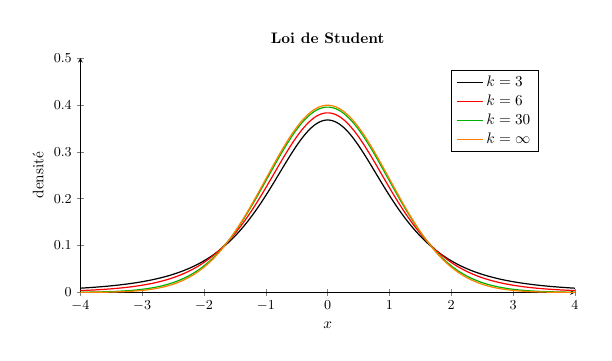
\begin{tikzpicture}[scale = 0.55]
\begin{axis}[
    domain=-4:4,
    samples=200,
    axis lines=left,
    ymin=0, ymax=0.5,
    xlabel={$x$},
    ylabel={densité},
    legend style={draw=black, fill=white, at={(0.75,0.95)}, anchor=north west},
    title={\textbf{Loi de Student}},
    width=13cm,
    height=7cm,
    tick label style={font=\small},
    legend cell align={left},
    scaled y ticks=false
]

% k = 3
\addplot[black, thick, domain=-4:4] 
  {0.3675526 * (1 + x^2/3)^(-2)};
\addlegendentry{$k=3$}

% k = 6
\addplot[red, thick, domain=-4:4] 
   {0.3827328 * (1 + x^2/6)^(-3.5)};
\addlegendentry{$k=6$}

% k = 30
\addplot[green!70!black, thick, domain=-4:4] 
  {0.3950100 * (1 + x^2/30)^(-15.5)};
\addlegendentry{$k=30$}

% k = infty
\addplot[orange, thick, domain=-4:4] 
  {1/sqrt(2*pi)*exp(-x^2/2)};
\addlegendentry{$k=\infty$}

\end{axis}
\end{tikzpicture}
\end{center}

\end{frame}



\begin{frame}[t]{Propriétés de la loi $t$}

{\small
\begin{itemize}
\item Si $T\sim t_v$ {\scriptsize (et $v>1$)}, alors $E(T) = 0$.
\item Si $T\sim t_v$ {\scriptsize (et $v>2$)}, alors $V(T) = \dfrac{v}{v-2}$.
\item Si $Z\sim N(0,1)$, $\quad K\sim\chi^2_v$, $\quad Z$ et $K$ sont indépendantes,
$$\text{alors}\quad \dfrac{Z}{\sqrt{K/v}}\sim t_v$$
% \item<3-> Si $X_1,\ldots,X_n$ sont i.i.d. $N(\mu,\sigma^2)$, alors
% $$\frac{\overline{X}-\mu}{S/\sqrt{n}}\sim t_{n-1}.$$
\end{itemize}
}
\end{frame}

\begin{frame}[t]{Table de la loi de Student}

\begin{minipage}[b]{2.5cm}{
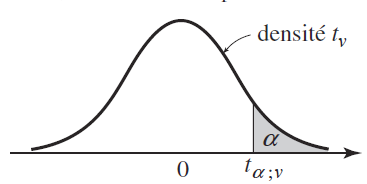
\includegraphics[width=2.5cm]{t-fig.PNG}

\vspace{9cm}}
\end{minipage}
\begin{minipage}[b]{7.6cm}{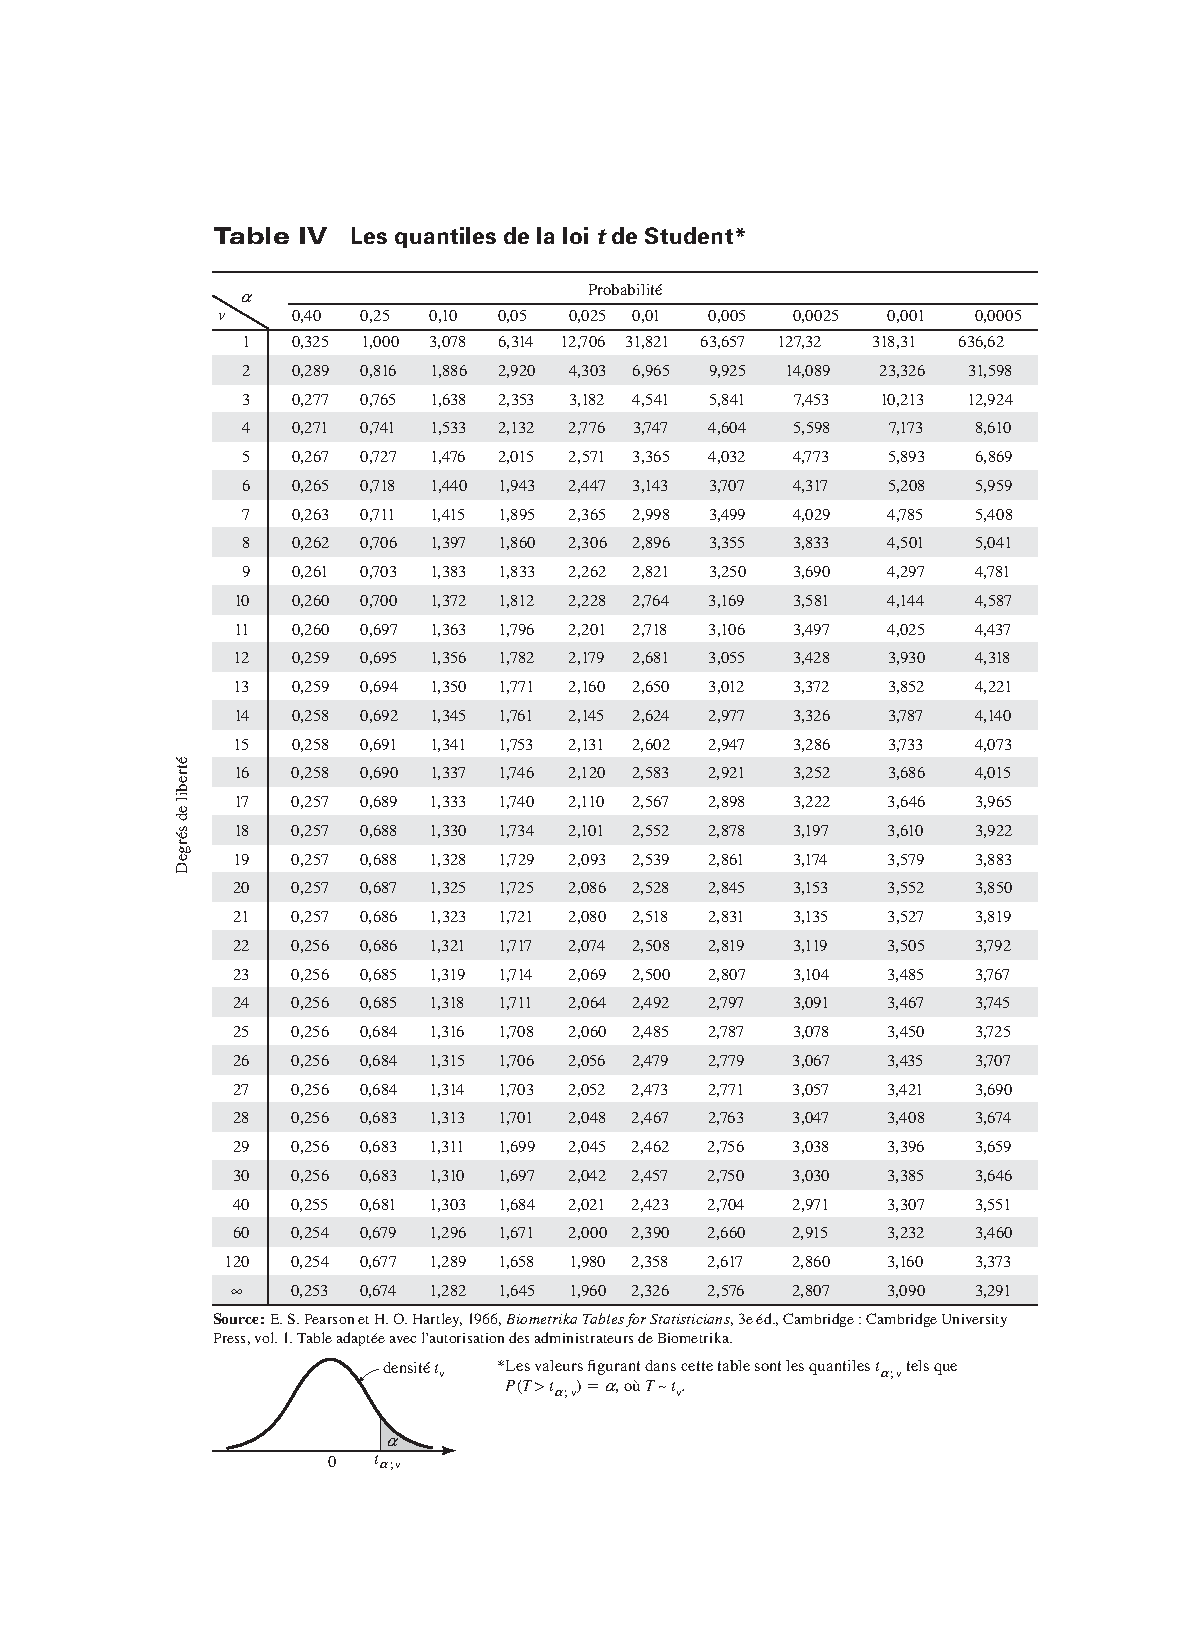
\includegraphics[width=7.6cm]{table_t.pdf}} \end{minipage}

\end{frame}

\begin{frame}[t]{Loi échantillonnale de $\overline{X}$, suite ...}
   Il est possible de démontrer que les propriétés précédentes mènent au résultat qui suit.
   \begin{Boite}{Loi échantillonnale de $\overline{X}$}
    Soit $X_1,\dots,X_n$ un échantillon aléatoire d'une loi $\mathcal{N}(\mu,\sigma^2)$. Alors
    $$\frac{\overline{X}-\mu}{S/\sqrt{n}}\sim t_{n-1}.$$
\end{Boite}

 \href{https://jmiron-stdsvsigma.share.connect.posit.cloud/}{Graphiquement}
\end{frame}

\begin{frame}[t]{Exemple 4}

{\small
On effectue 9 forages sur un terrain afin de déterminer la
profondeur à laquelle un certain minerai peut être extrait.

\begin{itemize}
\item $X_i=$ profondeur du minerai  lors du forage $i$.
\item On  suppose que les $X_i$ sont i.i.d. $N(\mu,\sigma^2)$.
    \end{itemize}

Quelle est la probabilité que la moyenne échantillonale soit supérieure à la vraie moyenne $\mu$ par plus d'un écart-type échantillonnal ?

}
\end{frame}


\section{Loi de Fisher}

\begin{frame}[t]{Loi échantillonnale de $S^2_1/S^2_2$}
   Si on veut comparer les variances de deux populations indépendantes de loi normale, il est logique de baser ces comparaisons sur le rapport des deux variances échantillonnales $S^2_1/S^2_2$. Nous aurons besoin de la loi de Fisher pour ce faire.
\end{frame}


\begin{frame}{Loi de Fisher (loi $F_{u,v}$)}

 \begin{itemize}
 \item Valeurs possibles de la variable: $[0,\infty)$
 \item Deux paramètres appelés\\"degrés de liberté au numérateur" ($u$), et  \\"degrés de liberté au dénominateur" ($v$).
\end{itemize}
\begin{center}
   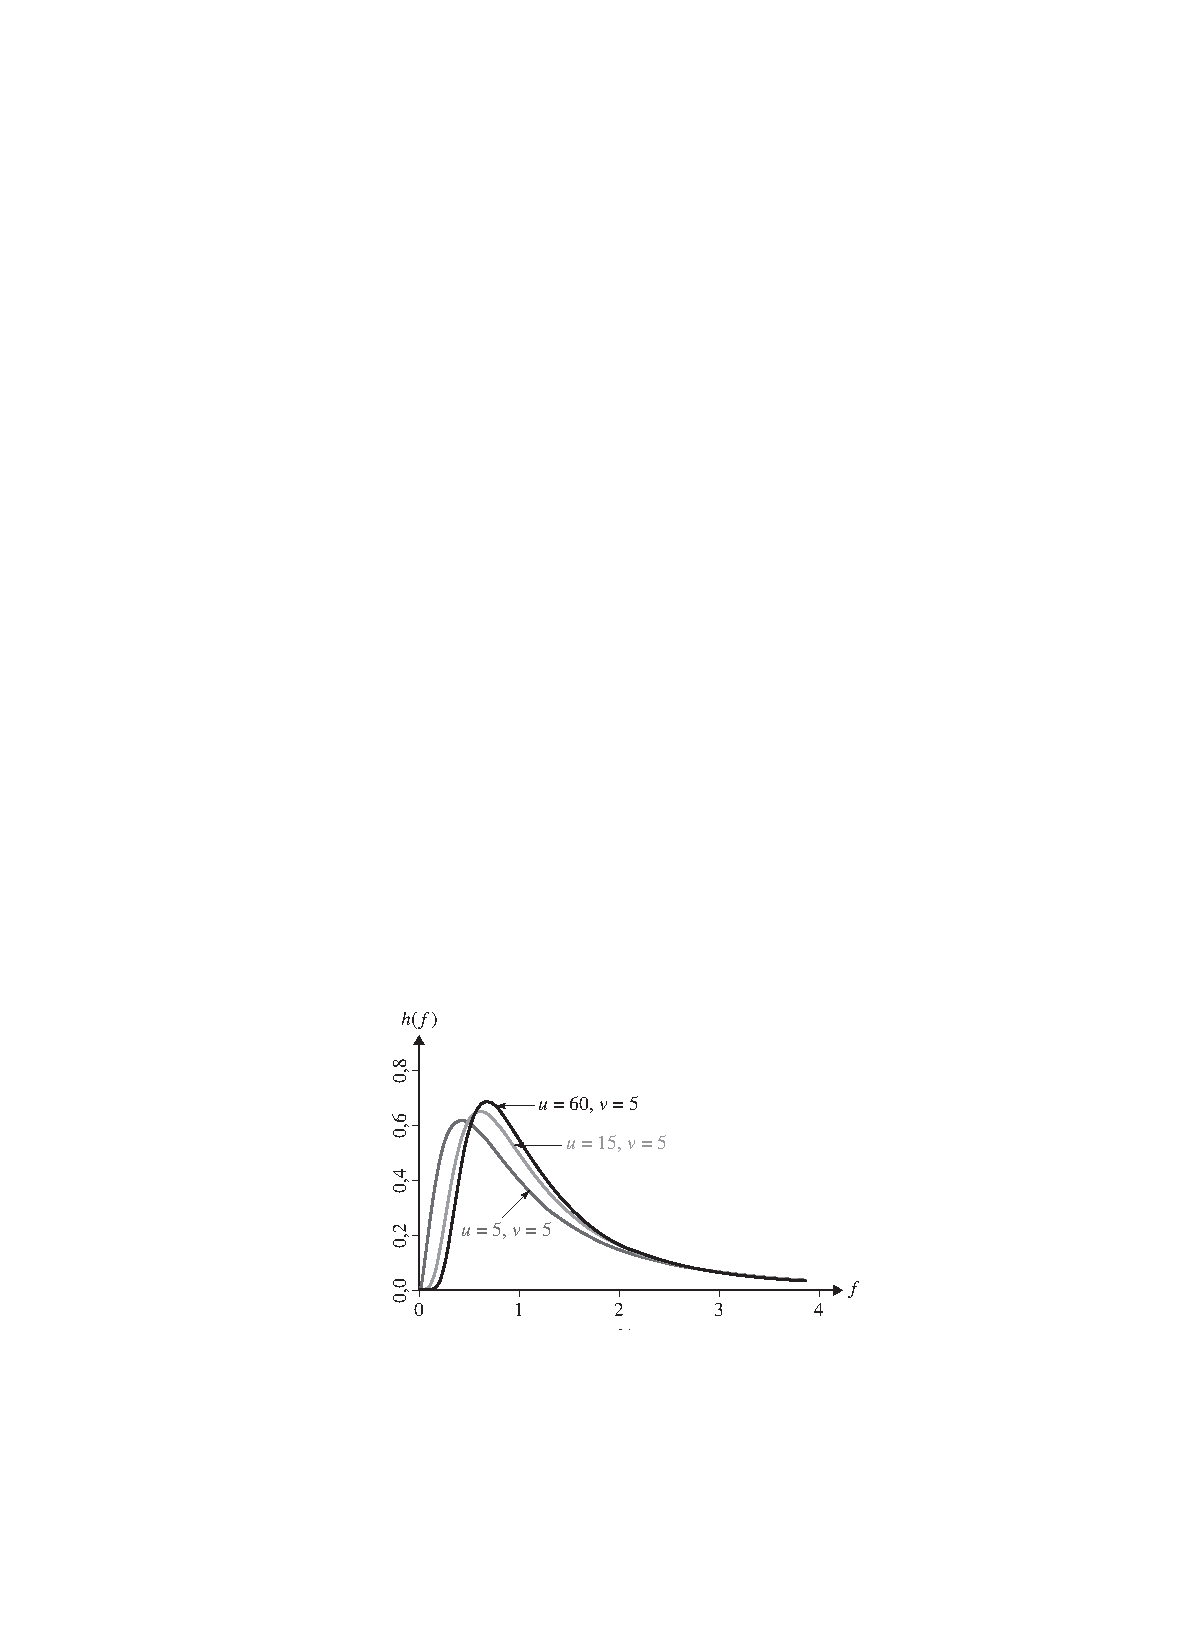
\includegraphics[width=5cm]{F_ddl_num.pdf}
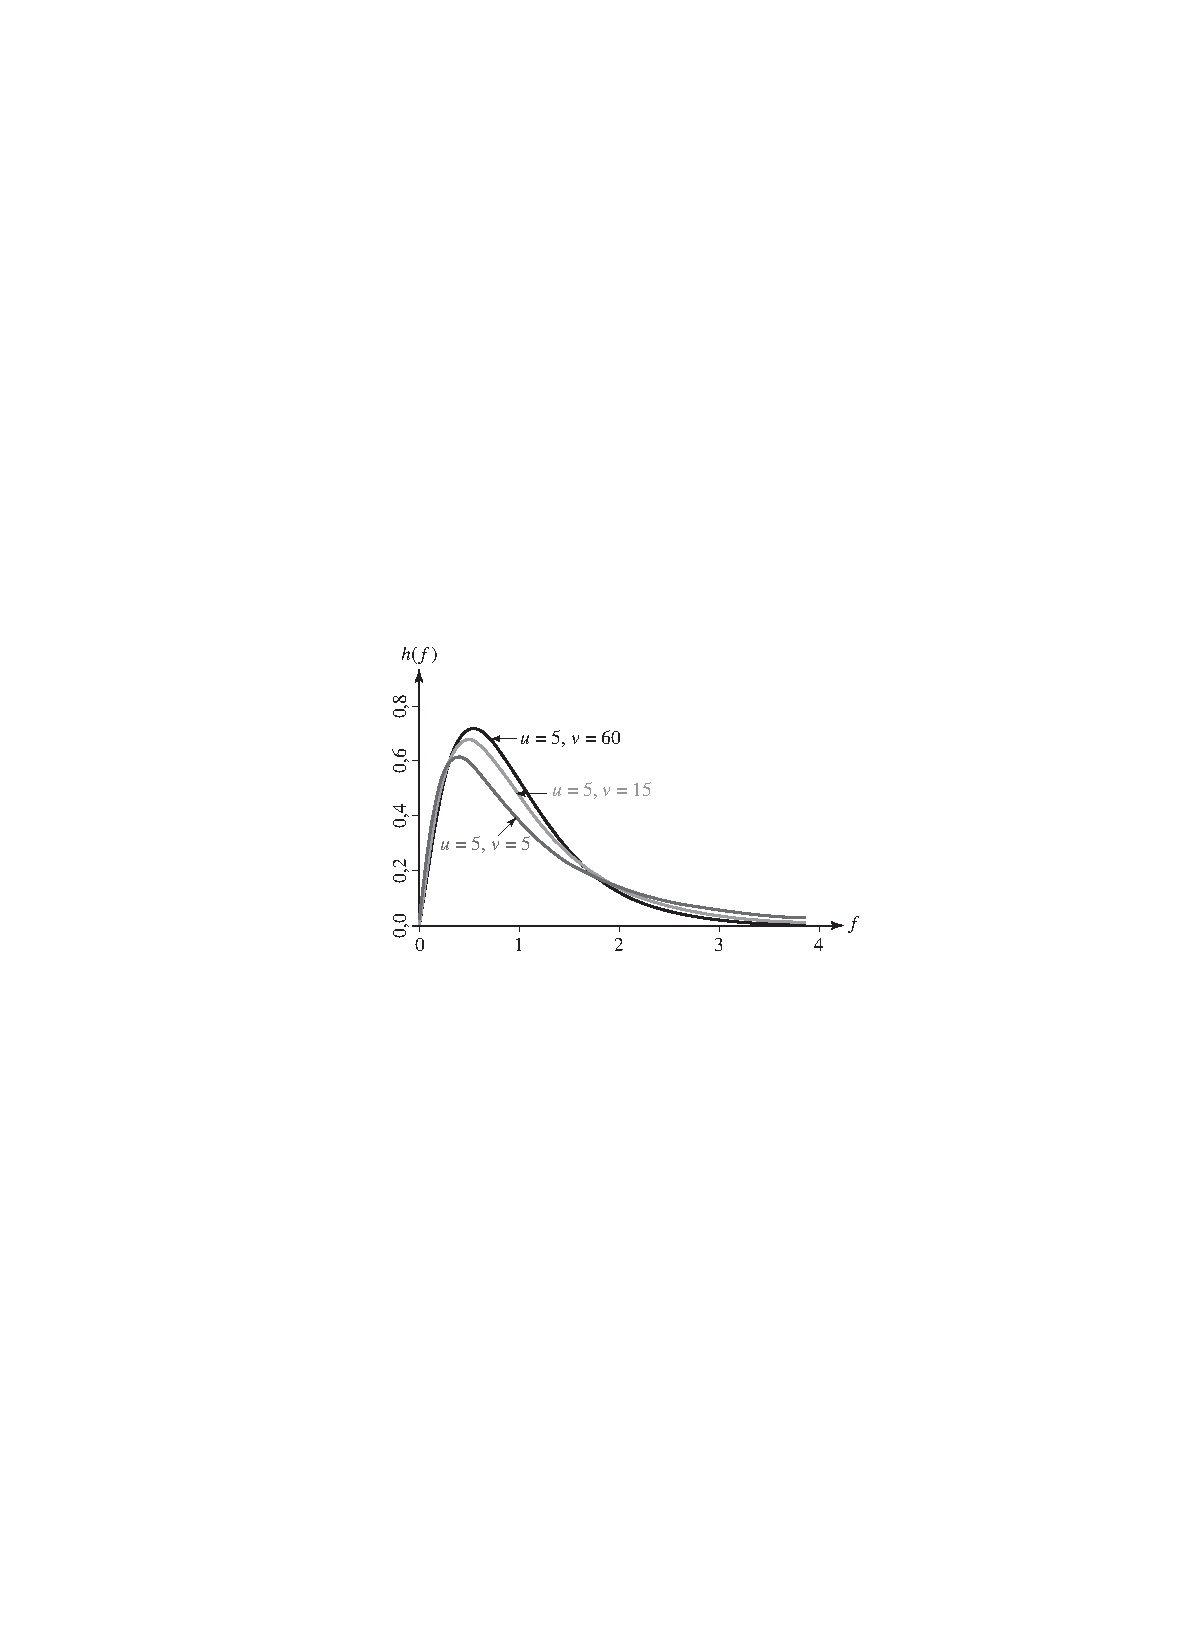
\includegraphics[width=5cm]{F_ddl_denom.pdf} 
\end{center}

\end{frame}

\begin{frame}[t]{Propriétés de la loi $F$}

{\small
\begin{itemize}
\item Si $F\sim F_{u,v}$ { (et $v>2$)}, alors $E(F) = \frac{v}{v-2}$;
\item si $F\sim F_{u,v}$ { (et $v>4$)}, alors  $V(F)= \dfrac{2v^2(u+v-2)}{u(v-2)^2(v-4)}$;
\item si $W\sim \chi^2_u$, $\quad K\sim\chi^2_v$, $\quad W$ et $K$ sont indépendantes, alors
$$\frac{W/u}{K/v} \sim F_{u,v}$$
\item si $Y\sim F_{u,v}$ alors $\dfrac{1}{Y}\sim F_{v,u}$.
\item si $T\sim t_{v}$ alors $T^2\sim F_{1,v}$.
\end{itemize}
}
\end{frame}

\begin{frame}[t]{Table de la loi de Fisher}

\begin{minipage}[b]{2.3cm}{
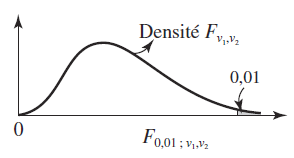
\includegraphics[width=2.3cm]{F01-fig.png}

\vspace{4cm}}
\end{minipage}
\begin{minipage}[b]{8cm}{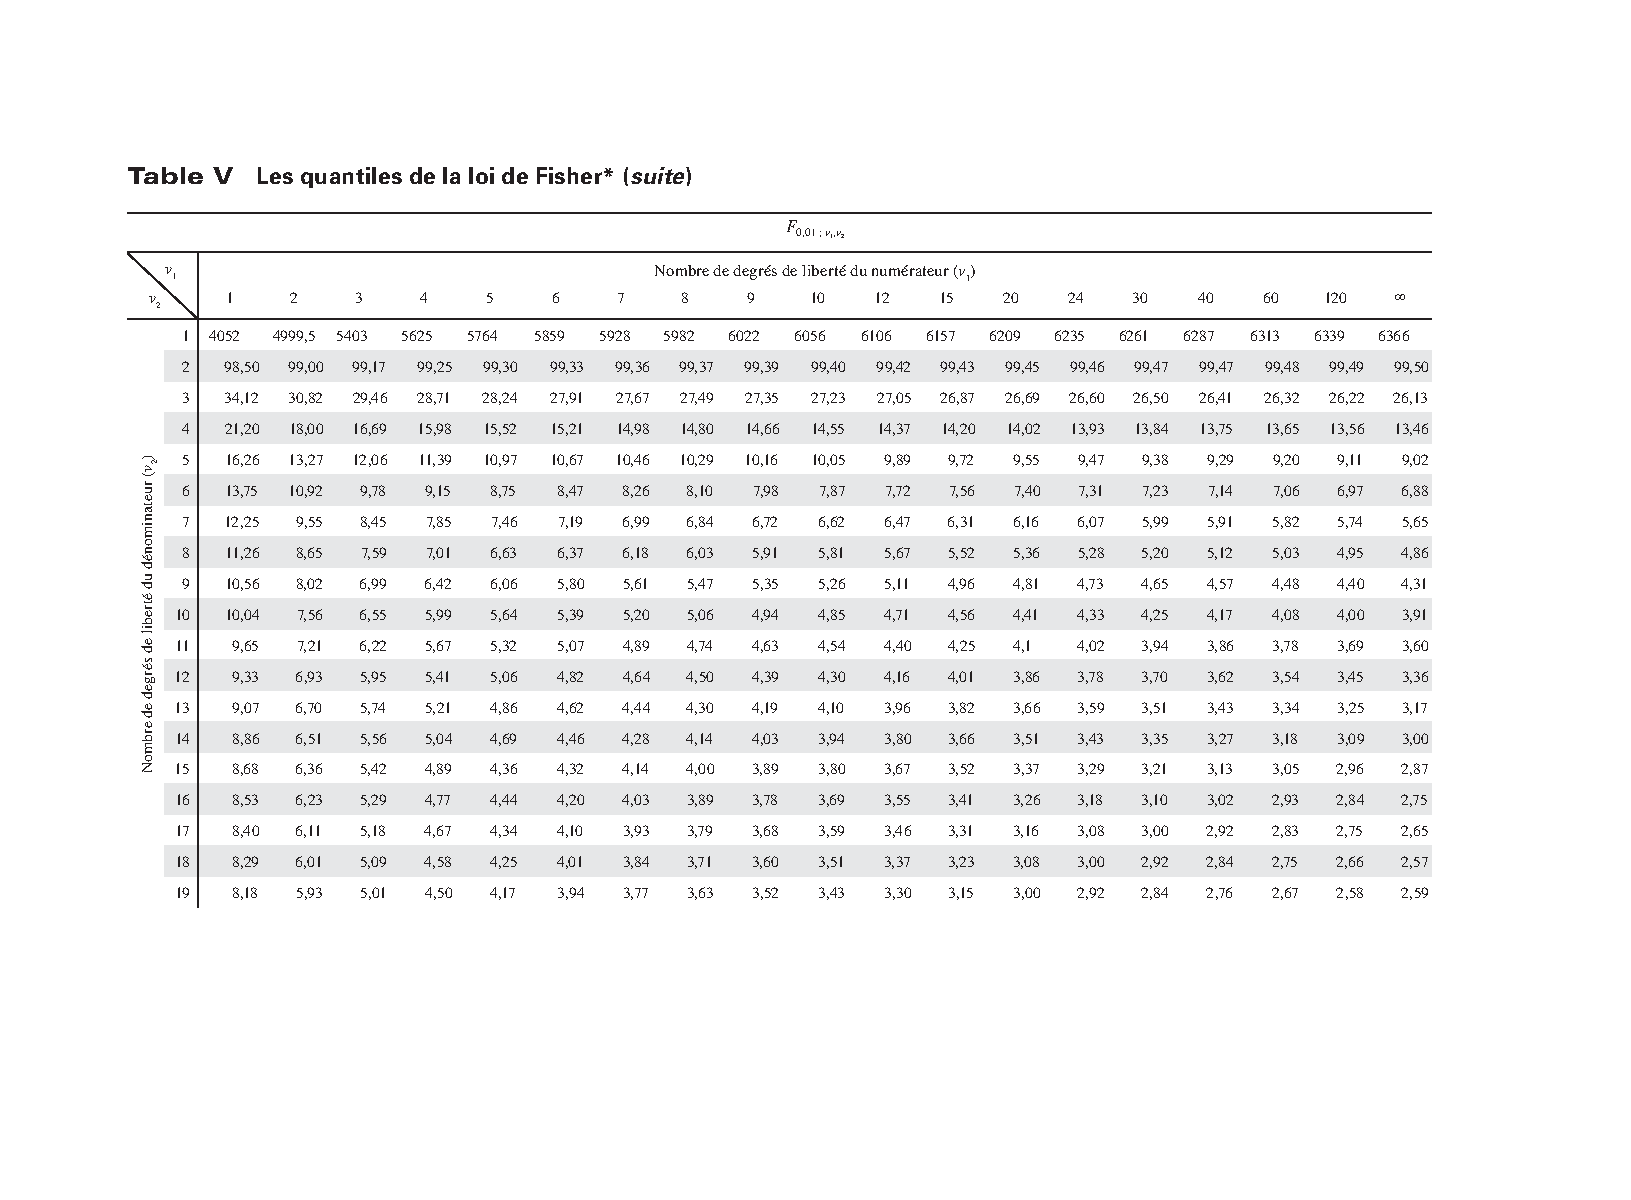
\includegraphics[width=10.5cm]{Fisher01_1.pdf}} \end{minipage}

%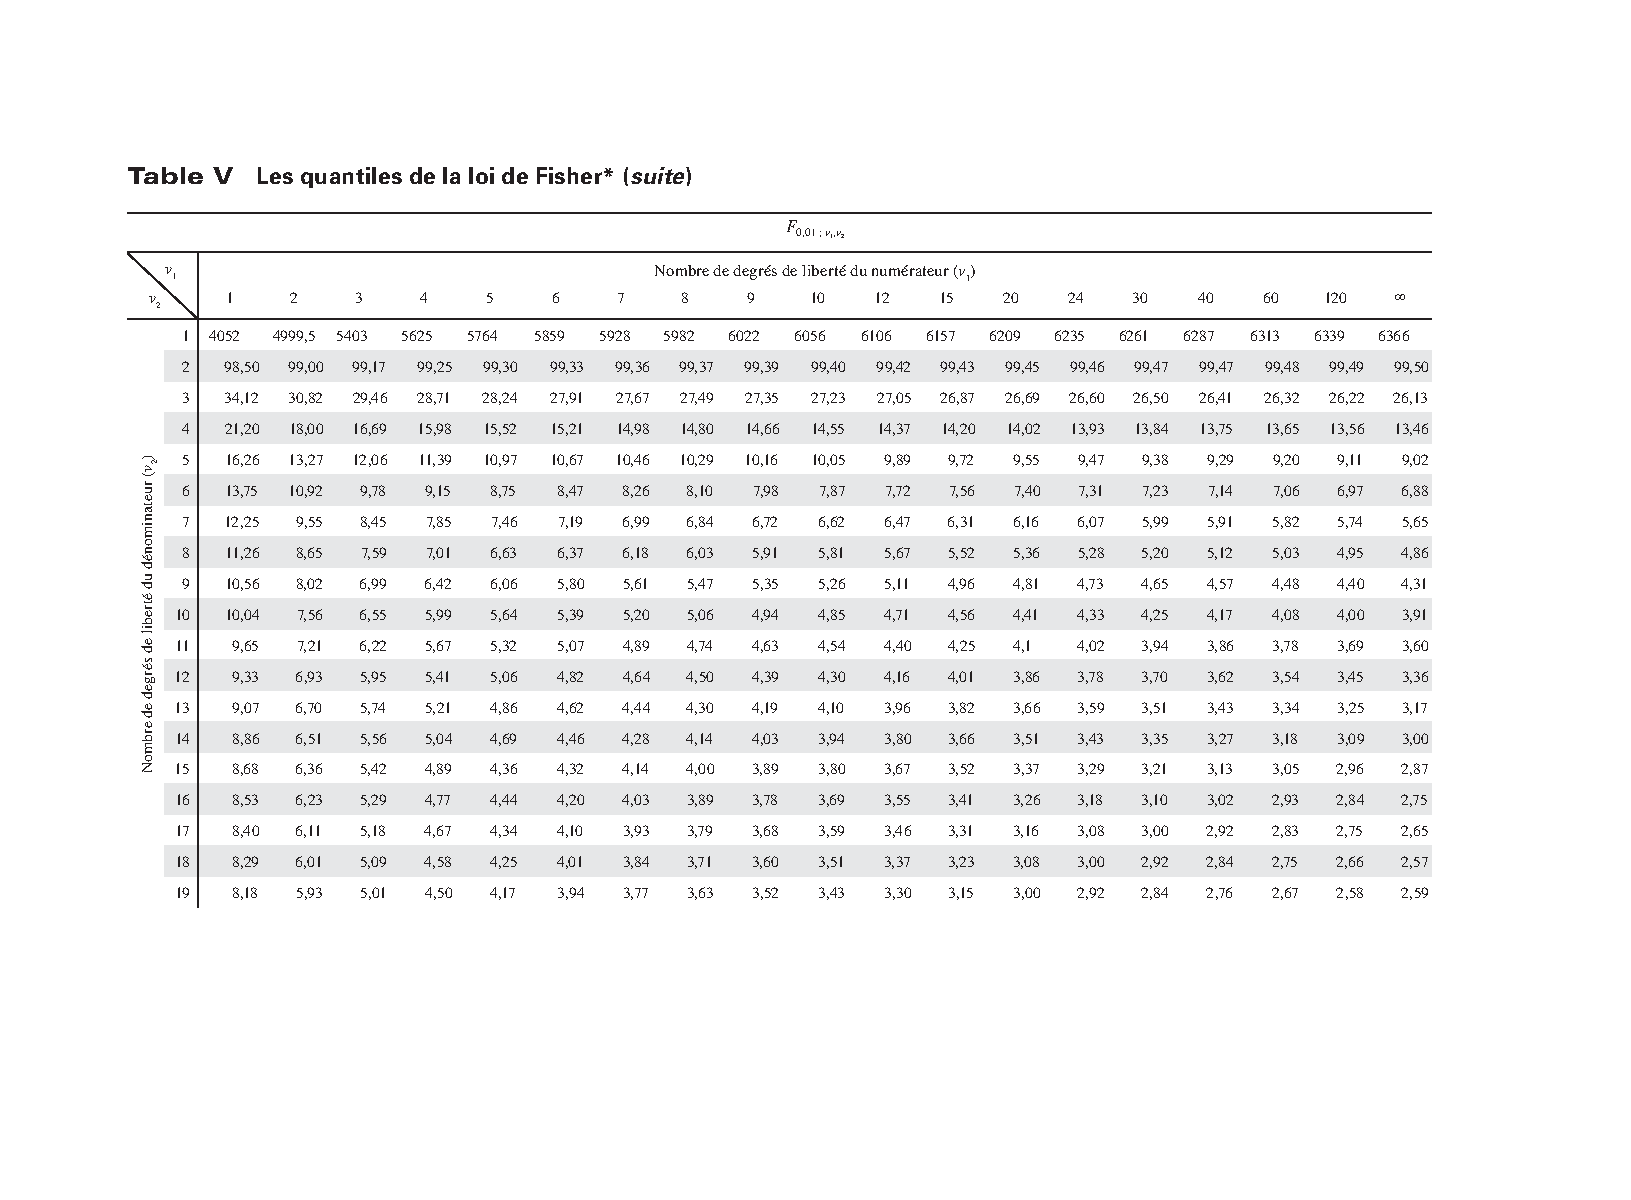
\includegraphics[width=10cm]{Fisher01_1.pdf}
\end{frame}



\begin{frame}[t]
 \frametitle{Exemple 5}

Trouver la valeur du quantile qui respecte les probabilités suivantes.
 \begin{itemize}
\item $P(F_{5,10}>a)=0,01$
\vspace{1cm}

\item $P(F_{5,10}<b)=0,01$

\vspace{2cm}
\item $P(F_{3,8}>c)=0,95$

\vspace{2cm}
\end{itemize}
\end{frame}


\begin{frame}{Loi échantillonnale de $S^2_X/S^2_Y$}

   \begin{Boite}{Loi échantillonnale de Loi échantillonnale de $S^2_X/S^2_Y$}
    Soit $X_1,\dots,X_{n}$ un échantillon aléatoire d'une loi $\mathcal{N}(\mu_X,\sigma_X^2)$
    et $Y_1,\dots,Y_{m}$ un échantillon aléatoire d'une loi $\mathcal{N}(\mu_Y,\sigma_Y^2)$,
    et supposons que ces deux échantillons sont indépendants. Soit $S^2_X$ la variance
    échantillonnale de $X_1,\dots,X_{n}$ et $S^2_Y$ la variance échantillonnale de $Y_1,\dots,Y_{m}$.
    Alors
    $$\frac{S^2_X/\sigma^2_X}{S^2_Y/\sigma^2_Y}\sim F_{n-1;m-1}.$$
\end{Boite}
 
\end{frame}



\begin{frame}[t]
 \frametitle{Exemple 6}

 {\small
Considérons deux échantillons indépendants.
\begin{itemize}
\item $1^{er}$ échantillon: $X_1,\ldots,X_6\sim N(\mu_X,\sigma_X^2)$ %(i.i.d.)
\item $2^e$ échantillon: $Y_1,\ldots,Y_{11}\sim N(\mu_Y,\sigma_Y^2)$ %(i.i.d.)
\item On vous dit que $\sigma^2_X=\sigma^2_Y=\sigma^2$.
\item $S^2_X$ et $S^2_Y$: les variances échantillonnales du $1^{er}$ et du $2^e$ échantillon, respectivement.
\end{itemize}

Quelle est la probabilité que $S^2_X \,>\,S^2_Y$?}

\end{frame}

 \begin{comment}
     

\section{Estimation ponctuelle}
\begin{frame}[t]{Exemple 1: MASSE ou RÉSISTANCE}

    \uncover<1->{Supposons que l'on s'intéresse à la résistance moyenne, $\mu$, des poutres d'un certain type qui sont fabriquées pour un nouveau pont.} 
    
    \uncover<2->{Nous ne pourrons jamais en connaître la vraie valeur, nous devrons l'estimer à partir d'un échantillon de taille $n$.}

    \uncover<3->{}
\end{frame}
\begin{frame}[t]{Exemple 1: masse des camions}

{\small
\begin{tabular}{l p{8cm}}
 {\bf Population :}& l'ensemble des camions qui passent sur un viaduc\\[4mm]
{\bf Caractéristique d'intérêt:}   &  $X$: masse d'un camion\\[4mm]
{\bf Modèle probabiliste :}& $X\sim N(\mu,\sigma^2)$\\[4mm]
{\bf Paramètre d'intérêt :}&  $\mu$: espérance du poids des camions qui passent sur ce viaduc\\[4mm]
{\bf Taille d'échantillon: }&  $n=30$\\[4mm]
{\bf Échantillon aléatoire:}&  $X_1,\,X_2,...,\,X_{30}$\\[4mm]
{\bf Échantillon  observé:}&  $x_1,\,x_2,...,\,x_{30}$\\[4mm]
{\bf Estimation ponctuelle :} &$\overline{x} $ tonnes
\end{tabular}
}
\end{frame}

\begin{frame}[t]{Exemple 1 VERSION 2: résistance des poutres d’acier}

{\small
\begin{tabular}{l p{8cm}}
 {\bf Population :}& L’ensemble des poutres d’acier fabriquées pour un nouveau pont.

\\[4mm]
{\bf Caractéristique d'intérêt:}   &  $X$: charge maximale (en kN) qu’une poutre peut supporter avant rupture.\\[4mm]
{\bf Modèle probabiliste :}& $X\sim N(\mu,\sigma^2)$\\[4mm]
{\bf Paramètre d'intérêt :}&  $\mu$: espérance de la charge maximale supportée par une poutre.\\[4mm]
{\bf Taille d'échantillon: }&  $n=30$\\[4mm]
{\bf Échantillon aléatoire:}&  $X_1,\,X_2,...,\,X_{30}$\\[4mm]
{\bf Échantillon  observé:}&  $x_1,\,x_2,...,\,x_{30}$\\[4mm]
{\bf Estimation ponctuelle :} &$\overline{x} $ kilonewtons (kN)
\end{tabular}
}
\end{frame}

 \end{comment}
\section{Estimation ponctuelle}

%\subsection{Introduction}

%%%%%%%%%%%%%%%%%%%%%%%%%%%%%%%%%%%%%%%%%%%%%%%%%%%%%%%%%%%%%%%%%%%%%%%%%%%%%%%%%%%%%%%%%%%
\begin{frame}[t]{Estimation : contexte}

\begin{itemize}
 \item<1-> Soit une variable aléatoire $X$ dont la répartition $F$ est caractérisée par $\theta$, un paramètre (ou un vecteur de paramètres) quelconque \textit{\textbf{inconnu}}. Par exemple la loi normale est caractérisée par son espérance $\mu$ et sa variance $\sigma^2$, dont l'un et/ou l'autre peuvent être des paramètres inconnus.

\item<2-> On recueille un échantillon aléatoire $X_1,\dots,X_n$ à partir de la loi de $X$.

\item<3-> Comme l'échantillon renferme de l'information sur $\theta$, on pourra extraire celle-ci en calculant une/des statistique(s) appropriée(s).
\end{itemize}
\end{frame}

\begin{frame}[t]{Estimation : définition d'un estimateur}
    Supposons que nous avons une variable aléatoire $X$ dont la répartition $F$ est caractérisée par $\theta$, un paramètre de valeur inconnue que nous voulons estimer.

    \begin{Boite}{Estimateur ponctuel}
        Soit $X_1,\hdots,X_n$, un échantillon aléatoire de la variable aléatoire $X$. Un estimateur de $\theta$ est une statistique $\hat{\theta}=T(X_1,\hdots,X_n)$.
    \end{Boite}
    
    \vfill
    Par exemple, la loi normale est caractérisée par son espérance $\mu$ et sa variance $\sigma^2$, qui sont des paramètres inconnus. Nous voudrons trouver deux statistiques, disons $\widehat{\mu}$ et $\widehat{\sigma}^2$, afin d'estimer les valeurs de $\mu$ et $\sigma^2$.
\end{frame}

\begin{frame}[t]{Loi échantillonnale vs bon estimateur}
\begin{itemize}
    \item<1-> Un estimateur est une statistique $\Rightarrow$ il existe une infinité d'estimateurs possibles !
    \item<2-> Un estimateur est une statistique $\Rightarrow$ un estimateur est une variable aléatoire. 
    \item<3-> Un bon estimateur devrait prendre une valeur ``proche'' de la vraie valeur de $\theta$ peu importe l'échantillon obtenu $\Rightarrow$ un bon estimateur a \alert{une loi échantillonnale  ``concentrée'' autour de la valeur de $\theta$}.
    \item<4-> Parmi l'infinité de statistiques possibles, on va tenter de trouver celle(s) dont la loi échantillonnale se ``concentre'' autour de $\theta$.
\end{itemize}
\end{frame}

\begin{frame}[t]{Qualités d'un estimateur}

    La statistique $\hat{\theta}$ est-elle la meilleure pour estimer $\theta$? \\


\begin{Boite}{Biais}
    Le biais de $\hat{\theta}$ pour $\theta$ est
    $$\text{Biais}(\hat{\theta}, \theta)=E(\hat{\theta})-\theta$$
\end{Boite}

Le biais quantifie donc la tendance de $\hat{\theta}$ à sur- ou sous-estimer
la valeur de $\theta$.

Un estimateur dont le biais est nul est dit ``sans biais'', et c'est ce que l'on recherche habituellement.
\end{frame}

\begin{frame}[t]{Qualités d'un estimateur}
    Plusieurs estimateurs sans biais peuvent exister pour le même paramètre. De deux estimateurs sans biais, on va privilégier celui qui varie le moins, donc qui a \alert{la plus faible variance}.

\medskip
    Et si deux estimateurs sont de biais différent ? \uncover<2->{Dans ce cas on privilégie
    celui qui fait la plus petite erreur d'estimation, en moyenne.

    \begin{Boite}{Erreur quadratique moyenne}
        \begin{align*}
        \text{EQM}(\hat{\theta}, \theta) &= E[(\hat{\theta}-\theta)^2] \\
                           &=V(\hat{\theta}) + [\text{Biais}(\hat{\theta},\theta)]^2
        \end{align*}
       \end{Boite}
       }
\end{frame}

\begin{frame}[t]{Comparaisons d'estimateurs}

   On quantifie la différence de performance entre deux estimateurs à l'aide
   de \alert{l'efficacité relative}.
    \begin{Boite}{Efficacité relative}
        Soit $\hat{\theta}_1$ et $\hat{\theta}_2$, deux estimateurs de $\theta$. L'efficacité relative de $\hat{\theta}_1$ par rapport à $\hat{\theta}_2$ est 

        $$\frac{\text{EQM}(\hat{\theta}_1, \theta)}{\text{EQM}(\hat{\theta}_2, \theta)}.$$
    \end{Boite}
\end{frame}



\section{Estimation de $\mu$ et $\sigma^2$}

\begin{frame}[t]{Paramètres classiques: $\mu$ et $\sigma^2$}

\begin{enumerate}[$\bullet$]\itemsep 1cm
\item<1-> Supposons que $X_1,\hdots,X_n$ proviennent d'une loi normale d'espérance $\mu$ et de variance $\sigma^2$, deux paramètres inconnus.
\item<2-> Par quelles quantités pourrait-on estimer $\mu$ et $\sigma^2$?

\item<3-> Calculons leurs biais et leurs erreurs quadratiques moyennes.
\end{enumerate}
\end{frame}

\begin{frame}[t]{Calcul du biais et de l'EQM de $\overline{X}$}
    
\end{frame}

\begin{frame}[t]{Calcul du biais et de l'EQM de $S^2$}
    
\end{frame}


\begin{frame}[t]{Comparons $S^2$ avec un autre estimateur}
 Plusieurs logiciels estiment $\sigma^2$ par
 $$\widehat{\sigma}^2=\frac{1}{n}\sum_{i=1}^n(X_i-\bar{X})^2.$$
 Calculons son biais et son EQM et comparons son efficacité relative à celle de $S^2$.

 [Aide : On a déjà fait ces calculs pour $S^2$, et $\widehat{\sigma}^2=(n-1)S^2/n$ ...]
\end{frame}

\begin{frame}[t]{Comparons $S^2$ avec un autre estimateur (suite)}

\end{frame}


\begin{comment}
    


\begin{frame}[t]{Qualités d'un estimateur}

 Le choix de \alert{$\overline X$} et \alert{$S^2$} est-il le meilleur pour estimer $\mu$ et $\sigma^2$? \\
 Quelles qualités devrait avoir un bon estimateur?\\

\begin{enumerate}\itemsep2cm
\item<1-> Être \alert{sans biais}, i.e. avoir une valeur espérée égale au paramètre estimé.
\item<2-> Avoir une \alert{variance faible}, idéalement qui diminue lorsque $n$ grandit.
\end{enumerate}
\end{frame}

\begin{frame}[t]{Estimation d'une moyenne $\mu$ par $\overline{X}$}
Soit $X_1,\ldots,X_n$ des variables aléatoires indépendantes d'espérance $\mu$ et de
variance $\sigma^2$. \\
Alors $ \overline{X} = \dfrac1n \sum\limits_{i=1}^{n}X_i$ est-il un bon estimateur de $\mu$?

\begin{itemize}
\item<1-> \alert{$\overline{X}$ est-il sans biais?} 
\vfill

\item<2-> \alert{$V(\overline{X})$ diminue-t-elle quand $n$ augmente?} 

\vfill
%\item<3-> $EQM(\hat{M} ) = \sigma^2/n$
\end{itemize}
\end{frame}

%\begin{frame}[t]{Estimation d'une proportion}
%Soit $X_1,\ldots,X_n$, des v.a. indépendantes et identiquement distribuées selon
%une loi de Bernoulli($p$). Alors
%$\hat{P}
%= \overline{X} = \sum\limits_{i=1}^{n}X_i/n=($nombre de $X_i$ égaux à 1$)/n$ est un bon
%estimateur de $p$:
%\begin{itemize}
%\item<1-> $\hat{P}$ est sans biais
%\item<2-> $Var(\hat{P}) = p(1-p)/n$
%\item<3-> $EQM(\hat{P} ) = p(1-p)/n$
%\end{itemize}
%\end{frame}
%
%\begin{frame}[t]{Exemple}
%
%{\small
%On veut estimer la proportion des roulements à billes provenant du
%fournisseur ABC qui sont défectueux. On prend un échantillon de 150
%roulements à billes au hasard parmi ceux provenant de ABC et on
%réalise que 15 d'entre eux sont défectueux. Donnez un estimé de la
%proportion des roulements à billes qui sont défectueux chez ABC.
%}
%\end{frame}


\begin{frame}[t]{Estimation d'une variance $\sigma^2$ par $S^2$}

Soit $X_1,\ldots,X_n$ des variables aléatoires indépendantes d'espérance $\mu$ et de
variance $\sigma^2$. \\
${S}^2 = \dfrac{1}{n-1}\sum\limits_{i=1}^{n}(X_i-\overline{X})^2$ est-il bon un estimateur de $\sigma^2$?

\begin{itemize}
\item<1-> \alert{${S}^2$ est-il sans biais?}
\vfill

\item<2-> \alert{$V({S}^2)$ diminue-t-elle quand $n$ augmente?}

\uncover<2->{On montrera plus tard que si les $X_i$ proviennent d'une loi normale, la variance de ${S}^2$ est $$V(S^2)=\dfrac{2\sigma^4}{n-1}.$$}
\end{itemize}

\end{frame}


\begin{frame}[t]{ }

\centerline{\LARGE\bf \alert{QUIZ !}}
\bigskip
On suppose que la taille des hommes canadiens suit une loi normale d'espérance 1,78 m et de variance $\sigma^2$.
\begin{itemize}
\item Hari mesure 250 Canadiens choisis au hasard.
\item Justine mesure 1000 Canadiens choisis au hasard.
\end{itemize}
\bigskip

{\bf Vrai ou Faux?}
\medskip

Hari a plus de chances que Justine d'obtenir...
\begin{itemize}
\item  une taille moyenne supérieure à 1,78 m.
\item  une taille moyenne supérieure à 1,82 m.
\end{itemize}


\vspace{1cm}

\end{frame}

\end{comment}
\begin{frame}[t]{Réponses aux exemples}

{\scriptsize
\begin{enumerate}
  \item Pas de question
  \item Quand $n$ augmente, la moyenne des $\overline x$ et des $s^2$ reste similaire, mais leur variance respective diminue. La distribution des $\overline x$ est symétrique, celle des $s^2$ est asymétrique, surtout pour des petits $n$.
  \item $P(S^2>54,4)=0,10$
  \item $P(\overline X>\mu+S)$ entre $0,005$ et $0,01$ (valeur exacte$=0,0085$)
  \item $a=5,64$, $b=0,0995$, $c=0,113$
  \item $P(S^2_X \,>\,S^2_Y)=0,465$
 \end{enumerate}
 }
\end{frame}
%Supposons deux v.a. indépendantes $U\sim\chi^2_5$ et $V\sim\chi^2_10$.
%On cherche
%\begin{align*}
%P(S^2_X>3.33S^2_Y)&=P\left[\frac{S^2_X}{S^2_Y}>3.33\right]
%=P\left[\frac{(5/\sigma^2)S^2_X}{(10/\sigma^2)S^2_Y}>\frac{(5/\sigma^2)}{(10/\sigma^2)}3.33\right]\\
%&=P\left[\frac{U}{V}>(0.5)(3.33)\right]=P\left[\frac{U/5}{V/10}>(0.5)(3.33)(10/5)\right]\\
%&=P(F_{5,10}>3.33)=0.05.
%\end{align*}
%\end{exemple}

\begin{comment}
\subsection{Propriétés des estimateurs}

\begin{frame}[t]{Plusieurs estimateurs possibles}

\alert{Toute fonction de l'échantillon} peut, en principe, servir d'estimateur pour un
paramètre $\theta$ donné. Mais clairement, certaines fonctions des
données semblent plus raisonnables que d'autres.

\medskip
Par exemple, dans l'exemple sur la grandeur des hommes de
20 ans on a pris $\hat{\Theta}_1 = \overline{X}$, mais on aurait également pu prendre
$\hat{\Theta}_2 = X_{28}$ ou $\hat{\Theta}_3 = (X_{(1)}+X_{(55)})/2$.

\bigskip
\uncover<2->{
{\bf Question générale :} Parmi l'infinité d'estimateurs disponibles
pour tout problème d'estimation, le(s)quel(s) devrait-on choisir ?
}
\end{frame}

\begin{frame}[t]{Estimateur sans biais}

\begin{block}{Définition}
Le biais d'un estimateur $\hat{\Theta}$ de $\theta$ est
$$\text{Biais}(\hat{\Theta}) = E[\hat{\Theta}]-\theta.$$
Un \alert{estimateur sans biais} est un estimateur de biais nul,
c'est-à-dire un estimateur tel que $E[\hat{\Theta}] = \theta$.
\end{block}
$\Rightarrow$ En moyenne, un estimateur sans biais n'a pas tendance à
sous-estimer ni sur-estimer le paramètre d'intérêt.

\smallskip
Biais$(\hat{\Theta}) < 0$ : $\hat{\Theta}$ a tendance à sous-estimer $\theta$.

\smallskip
Biais$(\hat{\Theta}) > 0$ : $\hat{\Theta}$ a tendance à sur-estimer $\theta$.
\end{frame}

\begin{frame}[t]{Retour à l'exemple}
Considérons $\hat{\Theta}_1 = \overline{X}$. Alors\\
$E[\hat{\Theta}_1] =$
\end{frame}

\begin{frame}[t]{Estimateur de faible variance}

{\small
Entre deux estimateurs de même biais, on va choisir celui qui a
\alert{la plus faible variance}.

S'ils sont de biais différents, alors on prend celui qui commet la
plus petite erreur (quadratique) d'estimation en moyenne (erreur
quadratique moyenne, EQM, la plus faible). Ce qui est
intéressant, c'est que l'EQM est une bonne mesure du
compromis biais/variance :\\
$EQM[\hat{\Theta}] =$
}
\end{frame}

\begin{frame}[t]{Un long exemple}
%On cherche à estimer la duree de vie d'un certain type de
%diodes. On pense que ces durées de vie sont distribuées selon
%une loi exponentielle de moyenne $\mu$. On recueille un échantillon
%aléatoire de 100 diodes et on mesure leurs durées de vie
%$X_1,\ldots,X_{100}$. Soit deux estimateurs
%$$
%\hat{M}_1 = \frac{X_1+\cdots+X_7}{7}
%\text{\ et\ }
%\hat{M}_2 = 2\times \frac{X_1+\cdots+X_{98}}{98}
%\times \frac{X_{99}}{X_{99}+X_{100}}.
%$$
%Lequel de ces deux estimateurs est préférable ? Quelle est son
%efficacité par rapport à l'autre? (Note : Vous pouvez utiliser le
%fait que $X_{99}/(X_{99}+X_{100})$ dans cet exemple précis suit une
%uniforme(0,1).)
\end{frame}

\begin{frame}[t]{Un long exemple (suite)}

{\ \ }
\end{frame}


\begin{frame}[t]{Un long exemple (suite)}

{\ \ }
\end{frame}

\end{comment}




\end{document}